\begin{exercise}
\begin{figure}[H]
\centering
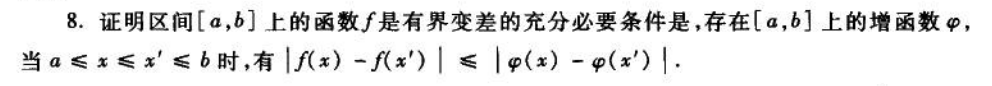
\includegraphics[width=\textwidth]{hw16-2025061715.png}
% \caption{}
\label{}
\end{figure}
\end{exercise}
\begin{proof}

\begin{theorem}[Jordan's theorem]
$f\in \text{BV}[a,b]$ iff $\exists$ increasing $f,g$ s.t. $f=g-h$.
\end{theorem}
\begin{proof}
$\Leftarrow$ is clear. $\Rightarrow$: $g(x)\coloneqq f(x)+\text{TV}(f_{[a,x]})$, $h(x)\coloneqq\text{TV}(f_{[a,x]})$, where $\text{TV}(f_{[a,x]})$ is the total variation function for $f$ over $[a,x]$.
\end{proof}

$\Rightarrow$: $\varphi:=g+h$, then
\[
\begin{aligned}
\lvert f(x)-f(x') \rvert & =\lvert g(x)-h(x)-g(x')+h(x') \rvert \\
 & \leq \lvert g(x)-g(x') \rvert+\lvert  h(x)-h(x')\rvert \\
 & =g(x')+h(x')-g(x)-h(x) \\
 & =\lvert \varphi(x)-\varphi(x') \rvert 
 \end{aligned}
\]
$\Leftarrow$: for partition $P\subset[a,b]$,
\[
\text{V}(f,P)=\sum_{P}\lvert f(x_{i+1})-f(x_i) \rvert \leq \sum_{P}\lvert \varphi(x_{i+1})-\varphi(x_i) \rvert =\sum_{P}(\varphi(x_{i+1})-\varphi(x_i))=\varphi(b)-\varphi(a)
\]
Then $\text{TV}(f)\leq\varphi(b)-\varphi(a)$ bounded. Thus $f\in\text{BV}[a,b]$.

\end{proof}

\begin{exercise}
\begin{figure}[H]
\centering
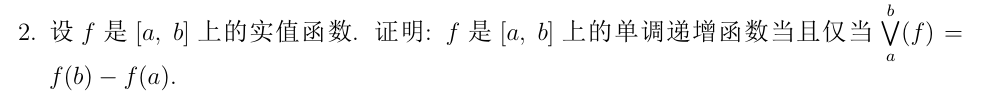
\includegraphics[width=\textwidth]{1-hw16-2025061715.png}
% \caption{}
\label{}
\end{figure}
\end{exercise}
\begin{proof}
$\Rightarrow$ is clear. $\Leftarrow$: if $f$ is not increasing function on $[a,b]$, then $\exists a\leq c<d\leq b$, s.t. $f(c)>f(d)$. Then
\[
\begin{aligned}
\bigvee_a^b(f) & \geq \lvert f(b)-f(d) \rvert +\underbrace{ \lvert f(d)-f(c) \rvert }_{ >0 } +\lvert f(c)-f(a) \rvert  \\
 & >\lvert f(b)-f(d)  \rvert +\lvert f(c)-f(a) \rvert \\
 & \geq f(b)\underbrace{ -f(d)+f(c) }_{ >0 }-f(a)  &  \text{drop the }\lvert \cdot \rvert\\
 & > f(b)-f(a)
\end{aligned}
\]
Thus $\bigvee_a^b(f)=f(b)-f(a)$ does not hold, which is a contradiction.
\end{proof}

\begin{exercise}[12 (2)]
\begin{figure}[H]
\centering
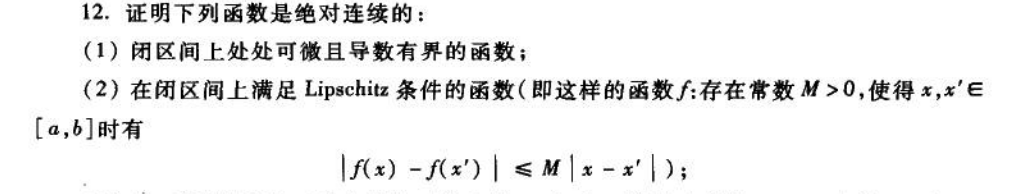
\includegraphics[width=\textwidth]{2-hw16-2025061715.png}
% \caption{}
\label{}
\end{figure}\label{73e14c}
\end{exercise}

\begin{proof}
(2) for any $\epsilon>0$, pick $\delta=\frac{\epsilon}{M}$, then for any disjoint $\{ (a_i,b_i) \}_{i=1}^{n}$ with $m\left( \bigcup_{i=1}^{n}(a_i,b_i) \right)<\delta$, we have
\[
\sum_{i=1}^{n} \lvert f(b_i)-f(a_i) \rvert \leq \sum_{i=1}^{n} M\lvert b_i-a_i \rvert < M\delta=\epsilon
\]
Therefore $f\in\text{AC}[a,b]$.
\end{proof}

\begin{exercise}
\begin{figure}[H]
\centering

\includegraphics[width=\textwidth]{3-hw16-2025061715.png}
% \caption{}
\label{}
\end{figure}
\end{exercise}
\begin{proof}
$\Rightarrow$: for $x\in[1,2]$ define $f (x)=f(1)$. For $f\in\text{Lip}[0,2]$, consider $\text{Diff}_{\frac{1}{n}}f(x)=n\left[ f\left( x+\frac{1}{n} \right)-f(x) \right]\leq n\cdot L\left[ \left( x+\frac{1}{n} \right)-x \right]=L$, which is bounded. As $f\in\text{Lip}[0,2]\subset\text{AC}[0,2]\subset\text{BV}[0,2]$, by Jordan's theorem and Lebesgue's Theorem, $f$ is the difference of two increasing function which is differentiable a.e. by Lebesgue's Theorem, thus $\text{Diff}_{\frac{1}{n}}f$ converges to $f'$ a.e. Claim that $\{ \text{Diff}_{h}f \}_{0<h\leq1}$ is uniformly integrable over $[0,2]$, then by Vitali Convergence theorem,
\[
\int_{0}^{x} f'(t) \, \mathrm{d}t=\lim_{ n \to \infty } \int_{0}^{x} \text{Diff}_{\frac{1}{n}}f(x) \, \mathrm{d}x =\lim_{ n \to \infty }\left[ n \int_{x}^{x+\frac{1}{n}} f(x) \, \mathrm{d}x-n\int_{0}^{\frac{1}{n}} f(x) \, \mathrm{d}x  \right] =f(x)-f(0)
\]
$f'$ is also bounded a.e., as for some $Z$ with measure 0, on $[0,2]\setminus Z$, $f'(x)=\lim_{ n \to \infty }\text{Diff}_{\frac{1}{n}}f(x)$, then for any $x$, $\exists N_{x}>0$, s.t. $\left\lvert  f'(x)-\text{Diff}_{\frac{1}{N_{x}}}f(x)  \right\rvert\leq1$, thus $\lvert f'(x) \rvert\leq \lvert \text{Diff}_{1/N_{x}}f(x) \rvert+\lvert f'(x)-\text{Diff}_{1/N_{x}}f(x) \rvert\leq L+1$. Define a bounded measurable function $\varphi$ that equals to $f'$ on $[0,2]\setminus Z$, and bounded by $L+1$ on $Z$. Then for any $x\in[0,1]$,
\[
\int_{0}^{x} \varphi(t) \, \mathrm{d}t = \int_{0}^{x} f'(t) \, \mathrm{d}t =f(x)-f(0)
\]
$\Leftarrow$: if for any $x\in[0,1]$, we have $\int_{0}^{x}\varphi=f(x)-f(0)$ for some bounded measurable $\varphi$. Let $M\coloneqq \sup_{x\in[0,1]}\lvert \varphi \rvert$. Then for any $0\leq x\leq y\leq1$,
\[
\lvert f(x)-f(y) \rvert =\left\lvert  \int_{0}^{x} \varphi-\int_{0}^{y} \varphi  \right\rvert =\left\lvert  \int_{x}^{y} \varphi  \right\rvert \leq \int_{x}^{y} \lvert \varphi \rvert \leq \int_{x}^{y} M=M(y-x)
\]
Thus $f\in\text{Lip}[0,1]$.
\end{proof}

\begin{exercise}
\begin{figure}[H]
\centering
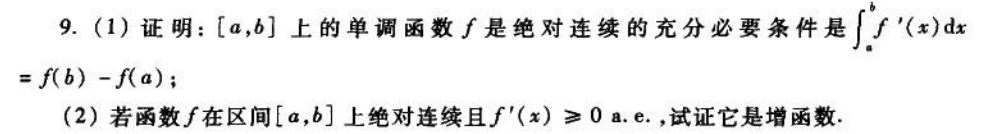
\includegraphics[width=\textwidth]{4-hw16-2025061715.png}
% \caption{}
\label{}
\end{figure}
\end{exercise}
\begin{proof}
(1)
$\Rightarrow$: is clear. $\Leftarrow$:

\begin{lemma}
For increasing $f$ on $[a,b]$, $\int_{a}^{b}f'\leq f(b)-f(a)$.
\end{lemma}
\begin{proof}
Let $f(x)\coloneqq f(b)$ for $x\in[b,b+1]$. Then
\[
\int_{a}^{b} f'=\lim_{ n \to \infty } \int_{a}^{b} \text{Diff}_{\frac{1}{n}}f=\lim_{ n \to \infty }n \left[ \int_{b}^{b+\frac{1}{n}}f-\int_{a}^{a+\frac{1}{n}} f  \right]=f(b)-\lim_{ n \to \infty } n\int_{a}^{a+\frac{1}{n}} \underbrace{ f }_{ \geq f(a) }\leq f(b)-f(a)
\]
\end{proof}
For any $x\in[a,b]$,
\[
f(b)-f(a)=\int_{a}^{b} f'=\int_{a}^{x} f'+\int_{x}^{b} f'\leq [f(x)-f(a)]+[f(b)-f(x)] =f(b)-f(a)
\]
then the equalities hold, i.e. $f(x)-f(a)=\int_{a}^{x}f'$ for any $x\in[a,b]$.

\begin{lemma}
A function $f\in\text{AC}[a,b]$ iff it's an indefinite integral over $[a,b]$.
\end{lemma}
\begin{proof}
$\Rightarrow$: is clear by the argument in \cref{73e14c}. $\Leftarrow$: for any $x\in[a,b]$,
\[
f(x)-f(a)=\int_{a}^{x} g
\]
for some $g\in L^{1}[a,b]$. Then $\forall\epsilon>0$, $\exists\delta>0$, s.t. $\int_{E}^{}\lvert g \rvert<\epsilon$ for any $E\subset[a,b]$ with $mE<\delta$. Then for any disjoint $\{ (a_i,b_i) \}_{i=1}^{n}$ with $m\left( \bigcup_{i=1}^{n}(a_i,b_i) \right)<\delta$, we have
\[
\sum_{i=1}^{n} \lvert f(a_i)-f(b_i) \rvert \leq \sum_{i=1}^{n} \left\lvert  \int_{a_i}^{b_i} g   \right\rvert \leq \sum_{i=1}^{n} \int_{a_i}^{b_i} \lvert g \rvert =\int_{\bigcup_{i=1}^{n} (a_i,b_i)}\lvert g \rvert \overset{ m\left( \bigcup_{i=1}^{n} (a_i,b_i) \right)<\delta }{ < }\epsilon
\]
Thus $f\in\text{AC}[a,b]$.
\end{proof}

Thus $f\in\text{AC}[a,b]$. We are done!

(2) in \cref{73e14c} we have proved the fundamental theorem of integral calculus. Then for any $a\leq x\leq y\leq b$,
\[
f(y)-f(x)=\int_{x}^{y} \underbrace{ f' }_{ \geq 0 }\geq 0
\]
i.e. $f$ is increasing on $[a,b]$.
\end{proof}

\begin{exercise}
\begin{figure}[H]
\centering
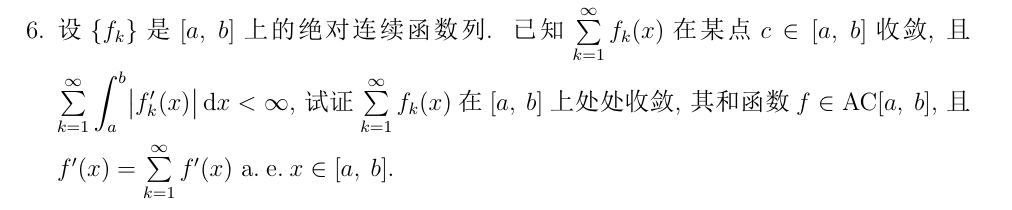
\includegraphics[width=\textwidth]{6-hw16-2025061715.png}
% \caption{}
\label{}
\end{figure}
\end{exercise}
\begin{proof}
$\forall\epsilon>0$, $\exists N>0$, s.t. $\sum_{k=N+1}^{\infty}\int_{a}^{b}\lvert f' \rvert<\epsilon/2$. For $k=1,\dots,N$, since $f_k\in\text{AC}[a,b]$, $\exists\delta>0$, s.t. for any disjoint $\{ (a_i,b_i) \}_{i=1}^{m}$ with $m\left[ \bigcup_{i=1}^{m}(a_i,b_i) \right]<\delta$, we have
\[
\sum_{i=1}^{m} \lvert f_k(a_i)-f_k(b_i) \rvert <\frac{\epsilon}{2N}
\]
\begin{note}
We can obtain $\delta _k$ for $k=1,\dots,N$ then let $\delta=\min_{1\leq k\leq N}\delta _k$.
\end{note}
Then
\[
\begin{aligned}
\sum_{i=1}^{m} \lvert f(a_i)-f(b_i) \rvert  & \leq \sum_{i=1}^{m} \sum_{k=1}^{\infty} \lvert f_k(a_i)-f_k(b_i) \rvert  \\
 & =\sum_{k=1}^{\infty} \sum_{i=1}^{m} \lvert f_k(a_i)-f_k(b_i) \rvert  & \text{by Tonelli theorem} \\
 & =\sum_{k=1}^{N} \underbrace{ \sum_{i=1}^{m} \lvert f_k(a_i)-f_k(b_i) \rvert }_{ \leq \epsilon/N } +\sum_{k=N+1}^{\infty} \underbrace{ \sum_{i=1}^{m} \lvert f_k(a_i)-f_k(b_i) \rvert }_{ =\sum_{i=1}^{m} \left\lvert  \int_{a_i}^{b_i} f'  \right\rvert \leq \sum_{i=1}^{m} \int_{a_i}^{b_i}\lvert f' \rvert=\int_{\bigcup_{i=1}^{m} (a_i,b_i)}^{} \lvert f' \rvert \leq \int_{a}^{b} \lvert f' \rvert    }  \\
 & \leq \epsilon/2+\sum_{k=N+1}^{\infty} \int_{a}^{b}\lvert f' \rvert  \\
 & \leq \epsilon/2+\epsilon/2  \\
 & \leq \epsilon
\end{aligned}
\]
Thus $f\in\text{AC}[a,b]$.

We need to show that for any $x\in[a,b]$,
\[
f(x)=f(a)+\int_{a}^{x} \sum_{k=1}^{\infty} f'_k
\]
$\forall\epsilon>0$, $\exists N>0$, s.t. $\int_{a}^{b}\sum_{k=N+1}^{\infty}\lvert f_k' \rvert<\epsilon/2$, then
\[
\left\lvert  \int_{a}^{x} \sum_{k=1}^{\infty} f_k' -\int_{a}^{x} \sum_{k=1}^{N} f'_k \right\rvert \leq \int_{a}^{b} \sum_{k=N+1}^{\infty} \lvert f_k' \rvert  \leq \frac{\epsilon}{2}
\]
\[
\begin{aligned}
\left\lvert  f(x)-f(a)-\sum_{k=1}^{N} (f_k(x)-f_k(a))  \right\rvert &  \leq \left\lvert  \sum_{k=N+1}^{\infty} (f_k(x)-f_k(a))  \right\rvert  \\
 & \leq \sum_{k=N+1}^{\infty} \int_{a}^{x} \lvert f_k' \rvert  \\
 & \leq \sum_{k=N+1}^{\infty} \int_{a}^{b} \lvert f'_k \rvert  \\
 & \leq \frac{\epsilon}{2}
\end{aligned}
\]
Therefore
\[
\begin{aligned}
 & \quad \left\lvert  f(x)-f(a)-\int_{a}^{x} \sum_{k=1}^{\infty} f_k'  \right\rvert  \\
 & =\left\lvert  f(x)-f(a)-\sum_{k=1}^{N} (f_k(x)-f_k(a))  \right\rvert +\left\lvert  \int_{a}^{x} \sum_{k=1}^{\infty} f_k' -\int_{a}^{x} \sum_{k=1}^{N} f'_k \right\rvert & \text{since }\int_{a}^{x} \sum_{k=1}^{N} f'_k=\sum_{k=1}^{N} (f_k(x)-f_k(a)) \\
 & \leq \frac{\epsilon}{2}+\frac{\epsilon}{2}=\epsilon
\end{aligned}
\]
Since $\epsilon$ is arbitrary, the conclusion is done!

\end{proof}

\begin{exercise}
\begin{figure}[H]
\centering
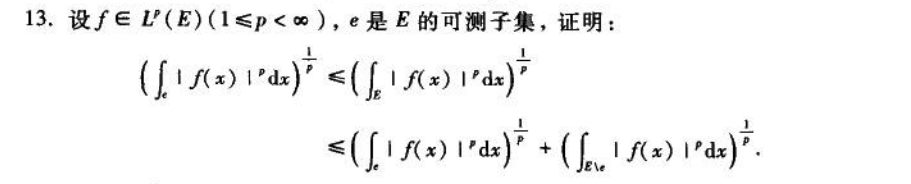
\includegraphics[width=\textwidth]{7-hw16-2025061715.png}
% \caption{}
\label{}
\end{figure}
\end{exercise}
\begin{proof}
\[
e\subset E\Rightarrow \int_{e}^{} \lvert f \rvert ^{p}\leq \int_{E}^{} \lvert f \rvert ^{p}
\]
By Jensen inequality, i.e. $(a+b)^{\frac{1}{p}}\leq a^{\frac{1}{p}}+b^{\frac{1}{p}}$ for $p\geq1$. Then
\[
\left( \int_{E}^{} \lvert f \rvert ^{p} \right)^{\frac{1}{p}}\leq \left( \int_{e}^{}\lvert f \rvert ^{p}+\int_{E\setminus e}^{} \lvert f \rvert ^{p}  \right)^{\frac{1}{p}}\leq \left( \int_{e}^{} \lvert f \rvert ^{p} \right)^{\frac{1}{p}}+\left( \int_{E\setminus e}\lvert f \rvert ^{p} \right)^{\frac{1}{p}}
\]
We are done!
\end{proof}

\begin{exercise}
\begin{figure}[H]
\centering
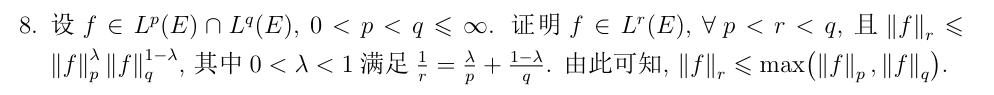
\includegraphics[width=\textwidth]{8-hw16-2025061715.png}
% \caption{}
\label{}
\end{figure}
\end{exercise}
\begin{proof}
(1) if $p=\infty$, then $\forall p<r<q$,
\[
\int_{E}\lvert f \rvert ^{r}\leq \int_{E}\lVert f \rVert _{\infty}^{r-p}\cdot \lvert f \rvert ^{p}=\lVert f \rVert _{\infty}^{r-p}\cdot \lVert f \rVert _{p}^{p}
\]
i.e.
\[
\lVert f \rVert _{r}\leq \lVert f \rVert _{\infty}^{1-\frac{p}{r}}\lVert f \rVert _{p}^{\frac{p}{r}}
\]
(2) if $p<\infty$, by Holder's inequality,
\[
\int_{E}^{} \lvert f \rvert ^{r}\leq \left( \int_{E}^{} \lvert f \rvert ^{ta} \right)^{\frac{1}{a}}\left( \int_{E}^{} \lvert f \rvert ^{sb} \right)^{\frac{1}{b}}
\]
we want $\frac{1}{a}+\frac{1}{b}=1,ta=p,sb=q,t+s=r$, i.e. $a=\frac{q-p}{q-r},b=\frac{q-p}{r-p}$. Then
\[
\int_{E}^{} \lvert f \rvert ^{r}\leq \left( \int_{E}^{} \lvert f \rvert ^{p} \right)^{\frac{q-r}{q-p}}\left( \int_{E}^{} \lvert f \rvert ^{q} \right)^{\frac{r-p}{q-p}}
\]
i.e.
\[
\lVert f \rVert _{r}\leq \lVert f \rVert _{p}^{\frac{p}{r}\frac{q-r}{q-p}}\cdot \lVert f \rVert_{q}^{\frac{q}{r}\frac{r-p}{q-p}}
\]
Let $\lambda=\frac{p}{r}\frac{q-r}{q-p}$, clearly $\frac{p}{r}\in (0,1),\frac{q-r}{q-p}\in (0,1)\Rightarrow\lambda\in(0,1)$, and $1-\lambda=\frac{q}{r}\frac{r-p}{q-p}$, $\frac{1}{r}=\frac{\lambda}{p}+\frac{1-\lambda}{q}$.
\end{proof}

\begin{exercise}
\begin{figure}[H]
\centering
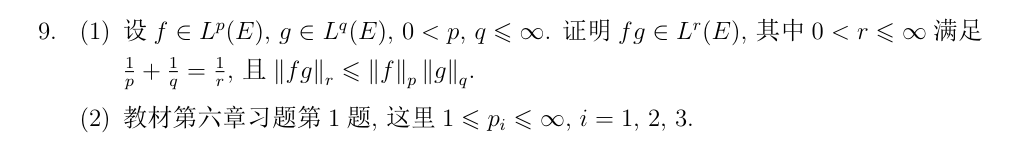
\includegraphics[width=\textwidth]{9-hw16-2025061715.png}
% \caption{}
\label{}
\end{figure}
\begin{figure}[H]
\centering
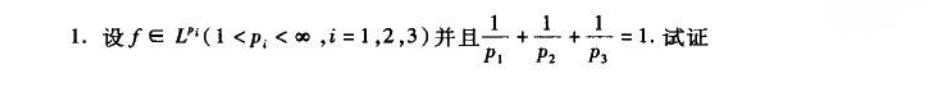
\includegraphics[width=\textwidth]{10-hw16-2025061715.png}
% \caption{}
\label{}
\end{figure}
\begin{figure}[H]
\centering
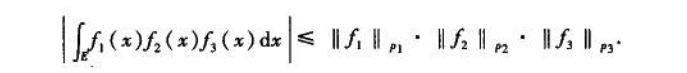
\includegraphics[width=\textwidth]{11-hw16-2025061715.png}
% \caption{}
\label{}
\end{figure}
\end{exercise}
\begin{proof}
(1) if $p=q=\infty$, then $r=\infty$, $\lVert fg \rVert_{\infty}\leq\lVert f \rVert_{\infty}\lVert g \rVert_{\infty}$. If $0<p<q=\infty$, then $r=p$, then $\lVert fg \rVert_{r}\leq \lVert g \rVert_{\infty}\lVert f \rVert_{p}$. If $0<p,q<\infty$,
\[
\int_{E}^{} \lvert fg \rvert ^{r}\leq \left( \int_{E}^{} \lvert f \rvert ^{p} \right)^{\frac{r}{p}}\left( \int_{E}^{} \lvert f \rvert ^{q} \right)^{\frac{r}{q}}
\]
i.e.
\[
\lVert fg \rVert _{r}\leq \lVert f \rVert _{p}\lVert g \rVert _{q}
\]
(2) if $p_2=p_3=\infty$, then $p_1=1$,
\[
\left\lvert  \int_{E}^{} f_1f_2f_3  \right\rvert \leq \int_{E}\lvert f_1f_2f_3 \rvert \leq \int_{E}^{} \lvert f_1 \rvert \cdot \lVert f_2 \rVert _{\infty}\cdot \lVert f_3 \rVert _{\infty}=\lVert f_1 \rVert _{\infty}\lVert f_2 \rVert _{\infty}\lVert f_3 \rVert _{\infty}
\]
If $p_3=\infty$, then $\frac{1}{p_1}+\frac{1}{p_2}=1$,
\[
\left\lvert  \int_{E}^{} f_1f_2f_3  \right\rvert\leq \int_{E}^{} \lvert f_1f_2f_3 \rvert \leq \lVert f_3 \rVert _{\infty}\int_{E}\lvert f_1f_2 \rvert \overset{ \text{Holder} }{ \leq  }\lVert f_1 \rVert _{p}\lVert f_2 \rVert _{q}\lVert f_3 \rVert _{\infty}
\]
If $p_3<\infty$, then $\frac{1}{p_1}+\frac{1}{p_2}=1-\frac{1}{p_3}$,
\[
\left\lvert  \int_{E}f_1f_2f_3  \right\rvert\leq \int_{E}^{} \lvert f_1f_2 \rvert \lvert f_3 \rvert \leq \lVert f_1f_2 \rVert _{\frac{1}{1-\frac{1}{p_3}}}\lVert f_3 \rVert _{p_3}\overset{ \text{9(1)} }{ \leq  }\lVert f_1 \rVert _{p_1}\lVert f_2 \rVert _{p_2}\lVert f_3 \rVert _{p_3}
\]
\end{proof}

\begin{exercise}
\begin{figure}[H]
\centering
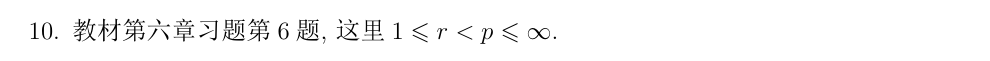
\includegraphics[width=\textwidth]{12-hw16-2025061715.png}
% \caption{}
\label{}
\end{figure}
\begin{figure}[H]
\centering
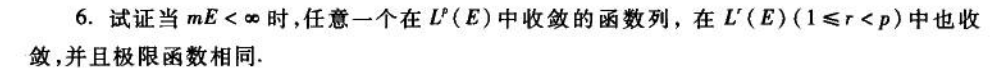
\includegraphics[width=\textwidth]{13-hw16-2025061715.png}
% \caption{}
\label{}
\end{figure}
\end{exercise}
\begin{proof}
If $p=\infty$, then $\lVert f_k-f \rVert_{\infty}\to0$, then $\lVert f_k-f \rVert_{r}\leq m(E)\cdot \lVert f_k-f \rVert_{\infty}\to0$.

If $p<\infty$, then by Holder inequality,
\[
\int_{E}^{} \lvert f_k-f \rvert ^{r}\leq \left( \int_{E}1 \right)^{\frac{p-r}{p}}\left( \int_{E}\lvert f_k-f \rvert ^{p} \right)^{\frac{r}{p}}
\]
i.e. $\lVert f_k-f \rVert_{r}\leq(mE)^{\frac{p-r}{pr}}\lVert f_k-f \rVert_{p}\to0$.
\end{proof}

\begin{exercise}
\begin{figure}[H]
\centering
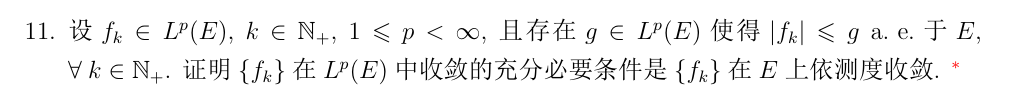
\includegraphics[width=\textwidth]{16-hw16-2025061715.png}
% \caption{}
\label{}
\end{figure}
\end{exercise}
\begin{proof}
By DCT, $\exists f\in L^{p}(E)$, s.t. $\lVert f_k \rVert_{p}\to \lVert f \rVert_{p}$.

$\Rightarrow$:
\[
m(E(\lvert f_k-f \rvert >\delta))\leq \int_{E(\lvert f_k-f \rvert >\delta)}^{} 1\leq \int_{E(\lvert f_k-f \rvert >\delta)}\left( \frac{\lvert f_k-f \rvert }{\delta} \right)^{p}\leq \frac{1}{\delta^{p}}\lVert f_k-f \rVert _{p}^{p}\to0
\]
$\Leftarrow$:
This is where the domination condition $\left(\left|f_k\right| \leq g\right.$ a.e. with $\left.g \in L^p(E)\right)$ is crucial.
Suppose $f_k \rightarrow f$ in measure on $E$.
Since $f_k \rightarrow f$ in measure, there exists a subsequence $\left\{f_{k_j}\right\}$ that converges pointwise almost everywhere to $f$.
Since $\left|f_k\right| \leq g$ a.e. for all $k$, it follows that $\left|f_{k_j}\right| \leq g$ a.e. for all $j$.
By Fatou's Lemma (or by taking the limit of the inequality), we can also show that $|f| \leq g$ a.e. To see this, consider any subsequence $f_{k_j}$ that converges a.e. to $f$. Then $\left|f_{k_j}\right| \rightarrow|f|$ a.e. and $\left|f_{k_j}\right| \leq g$ a.e. Thus, $0 \leq|f(x)| \leq g(x)$ a.e. for $x \in E$.
Since $g \in L^p(E)$, we have $\int_E g^p d \mu<\infty$. From $|f| \leq g$ a.e., it follows that $|f|^p \leq g^p$ a.e., so $\int_E|f|^p d \mu \leq \int_E g^p d \mu<\infty$, which means $f \in L^p(E)$.

Now, we want to show that $f_k \rightarrow f$ in $L^p(E)$, i.e., $\lim _{k \rightarrow \infty} \int_E\left|f_k-f\right|^p d \mu=0$.
Since $f_k \rightarrow f$ in measure, we know that for any subsequence $\left\{f_{k_j}\right\}$, there exists a further subsequence $\left\{f_{k_{j l}}\right\}$ that converges pointwise a.e. to $f$.
For this subsequence, we have:

\begin{enumerate}
	\item $f_{k_{j_l}} \rightarrow f$ a.e.
	\item $\left|f_{k_{j l}}-f\right|^p \leq\left(\left|f_{k_{j l}}\right|+|f|\right)^p \leq(g+g)^p=(2 g)^p=2^p g^p$ a.e. Since $g \in L^p(E)$, we have $2^p g^p \in L^1(E)$. Therefore, by the Dominated Convergence Theorem,
\end{enumerate}
\[
\lim _{l \rightarrow \infty} \int_E\left|f_{k_{j_l}}-f\right|^p d \mu=\int_E \lim _{l \rightarrow \infty}\left|f_{k_{j_l}}-f\right|^p d \mu=\int_E 0 d \mu=0
\]
This shows that every subsequence of $\left\{f_k\right\}$ has a further subsequence that converges to $f$ in $L^p(E)$. This implies that the entire sequence $\left\{f_k\right\}$ converges to $f$ in $L^p(E)$. If a sequence does not converge to a limit $L$, then there exists some subsequence that stays outside of any neighborhood of $L$. However, if every subsequence has a further subsequence that converges to $L$, then the original sequence must converge to $L$.
\end{proof}

\begin{exercise}
\begin{figure}[H]
\centering
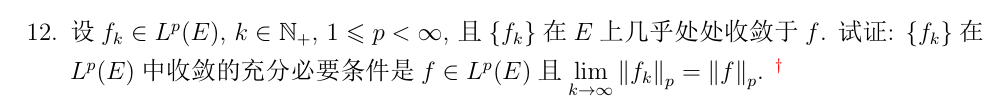
\includegraphics[width=\textwidth]{17-hw16-2025061715.png}
% \caption{}
\label{}
\end{figure}
\end{exercise}
\begin{proof}
$\Rightarrow$: $\lVert f \rVert_{p}\leq \lVert f_k-f \rVert_{p}+\lVert f_k \rVert_{p}\leq1+\lVert f_k \rVert_{p}<\infty$ for some large $k$. Then $f\in L^{p}(E)$. And
\[
\lvert \lVert f_k \rVert _{p}-\lVert f \rVert _{p} \rvert \leq \lVert f_k-f \rVert _{p}\to0
\]
Thus $\lim_{ k \to \infty }\lVert f_k \rVert_{p}=\lVert f \rVert_{p}$.

$\Leftarrow$: by Fatou's lemma,
\[
\varlimsup_{ k \to \infty } \int_{E}^{} \lvert f_k-f \rvert ^{p}\leq \int_{E}\underbrace{ \varlimsup_{ k \to \infty } \lvert f_k-f \rvert ^{p} }_{ =0\text{ a.e. } }=0
\]
then $\lVert f_k-f \rVert\to 0$.

\end{proof}
\begin{figure}[H]
\centering
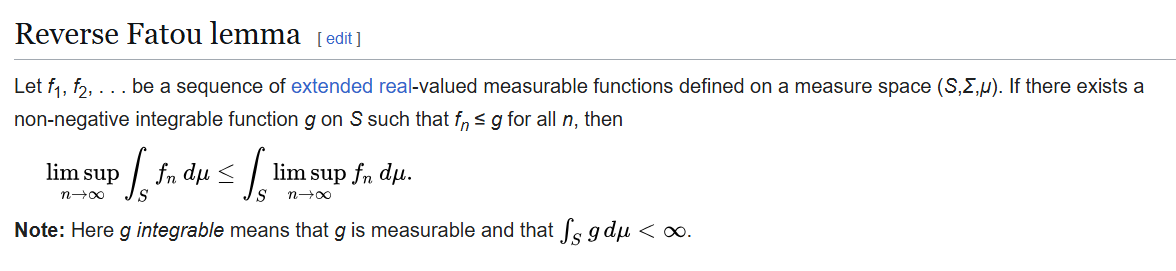
\includegraphics[width=\textwidth]{hw16-2025062009.png}
% \caption{}
\label{}
\end{figure}
